\section{Численные методы решения задачи Коши: метод Тейлора, методы Адамса.}

\subsection*{Метод Тейлора}

Решаем задачу Коши $\begin{cases}
    y'(x)=f(x,y) \\ y(0)=y^0
  \end{cases}$
Мы хотим построить наше решение в точках $y(h),y(2h)\ldots$,
предлагается явно посчитать значения в этих точках,
разложив в ряд Тейлора до $p+1$ степени. Далее для упрощения записи $y\defeq y(x_0),\ f\defeq f(x_0,y(x_0))$:
\[\begin{cases}
    y(x)=y+hy'+\frac{h^2}{2}y''+\sum_{s=2}^{p}y^{(s)}\frac{h^s}{s!}+\bigO(h^{p+1}) \\
    y'=f \text{ -- по условию}                                                     \\
    y''=f_x+f_yy'                                                                  \\
    y'''=f_{xx}+f_{xy}y'+f_{yx}y'+f_{y}y''+f_{yy}(y')^2                            \\
    \cdots
  \end{cases}
\]

Метод применим если $|x-x_0|$ больше области сходимости ряда Тейлора,
иначе предлагается разбивать отрезки на подотрезки и строить решение
в точке $x$ за несколько шагов.

\begin{remark}
  Данный алгоритм может быть полезен, когда требуется решить
  большое количество задач вполне определенного вида с
  различными начальными данными. В этом случае требуемые
  производные можно найти аналитически и сохранить для многократного
  применения.
\end{remark}

\begin{example}
  Решаем задачу $y'(x)=x^2\sin(y(x))$. Мы можем посчитать
  \begin{align*}
    y''(x) & = 2x\sin(y(x))+x^2\cos(y(x))y'(x)      \\
           & = 2x\sin(y(x))+x^4\cos(y(x))\sin(y(x))
  \end{align*}
  Таким образом второй порядок \textit{локальной} точности используя следующую формулу
  \[y_{k+1}=y_k+hx_k^2\sin(y_{k})+\frac{h^2}{2}[2x_k\sin(y_k)+x_k^4\cos(y_k)\sin(y_k)]\]
  Можно продолжать считать производные и получать более точный результат.
\end{example}

\begin{remark}
  Заметим, что здесь нет речи о разностной схеме, так как формально достаточно
  затруднительно посчитать \textit{глобальную} погрешность аппроксимации.
  Если при первом шаге мы считаем производную в известной нам начальной точке,
  то при каждом следующем шаге мы будем искать производную в точке, которая
  никак не привязана к изначальному уравнению.
\end{remark}

\subsection*{Методы Адамса первого порядка точности}

Решаем задачу Коши $\begin{cases}
    y'(x)=f(x,y) \\ y(0)=y^0
  \end{cases}$

Основная идея берется из точного равенства $y'(x_{k+1})\equiv y(x_k)+\int_{x_k}^{x_{k+1}}y'(x)dx=y(x_k)+\int_{x_k}^{x_{k+1}}f(x,y)dx$.
Различные методы Адамса возникают из разных способов взять интеграл

\begin{lemma}
  Пусть $g\in C^k[a,b],\ I(g)=\int_a^bg(x)dx$, тогда
  \begin{flalign*}
    & 1) \abs{I(g)-g(a)(b-a)}\leq \norm{g'}\frac{(b-a)^2}{2} \\
    & 2) \abs{I(g)-g(b)(b-a)}\leq \norm{g'}\frac{(b-a)^2}{2} \\
    & 3) \abs{I(g)-g\left(\frac{a+b}{2}\right)(b-a)}\leq\norm{g''}\frac{(a - b)^3}{24}    \\
    & 4) \abs{I(g)-\frac{g(a)+g(b)}{2}(b-a)}\leq\norm{g''}\frac{(b-a)^3}{12} \\
  \end{flalign*}
\end{lemma}
\begin{proof}
  Первые три неравенства берутся из разложения подынтегральной функции в ряд Тейлора
  с остаточным членом в форме Лагранжа в указанных точках:
  \begin{flalign*}
    & 1) \abs{\int_a^bg(a)+g'(\xi)(x-a)dx-g(a)(b-a)}=\abs{\int_a^bg'(\xi)(x-a)dx}\leq\norm{g'}\int_a^b(x-a)dx\leq\norm{g'}\frac{(b-a)^2}{2} \\
    & 2) \abs{\int_a^bg(b)+g'(\xi)(x-b)dx-g(b)(b-a)}=\abs{\int_a^bg'(\xi)(x-b)dx}\leq\norm{g'}\int_a^b(b-x)dx\leq\norm{g'}\frac{(b-a)^2}{2}                 \\
    & 3) \abs{\int_a^bg\left(\frac{a+b}{2}\right)+g'\left(\frac{a+b}{2}\right)\left(x-\left(\frac{a+b}{2}\right)\right)+\frac{g''(\xi)}{2}\left(x-\left(\frac{a+b}{2}\right)\right)^2dx-g\left(\frac{a+b}{2}\right)(b-a)}=    \\
    & \: \abs{\int_a^bg\left(\frac{a+b}{2}\right)dx+\underbrace{\int_a^bg'\left(\frac{a+b}{2}\right)\left(x-\left(\frac{a+b}{2}\right)\right)dx}_{=\ 0,\ (\text{симм. отн. середины})}+\int_a^b\frac{g''(\xi)}{2}\left(x-\left(\frac{a+b}{2}\right)\right)^2dx-g\left(\frac{a+b}{2}\right)(b-a)} \\
    & = \abs{\int_a^b\frac{g''(\xi)}{2}\left(x-\left(\frac{a+b}{2}\right)\right)^2dx}\leq \frac{\norm{g''}}{2}\abs{\int_a^b\left(x-\left(\frac{a+b}{2}\right)\right)^2dx}=\norm{g''}\frac{(a - b)^3}{24}
  \end{flalign*}
  Для доказательства 4ого пункта рассматриваем следующий интеграл
  \begin{multline*}
    \frac{1}{2}\int_a^bg''(x)(x-a)(x-b)dx= \frac{1}{2}g'(x)(x-a)(x-b)|_a^{b}-\frac{1}{2}\int_a^bg'(x)((x-b)+(x-a))dx= \\
    = -\frac{1}{2}g(x)((x-b)+(x-a))|_a^b +\int_a^bg(x)dx=\int_a^bg(x)dx-\frac{g(a)+g(b)}{2}(b-a)
  \end{multline*}
  Доказали эквивалентность предложенного интеграла, оценим его:
  \[\abs{\frac{1}{2}\int_a^bg''(x)(x-a)(x-b)dx}\leq\frac{\norm{g''}}{2}\abs{\int_a^bg''(x)(x-a)(x-b)dx}\leq\frac{\norm{g''}}{12}(b-a)^3\]
\end{proof}

\subsubsection*{Явный метод Эйлера}

Разностная схема получается из пункта 1) доказанной выше леммы:
\[\frac{y_{k+1}-y_k}{h}= f(x_k,y_k) + \bigO(h),\ y_0=y(x_0)\]
Локальная погрешность $O(h^2)$, глобальная погрешность и сходимость $O(h)$.

\begin{figure}[h]
  \centering
  \tikzsetnextfilename{13/ExplicitEuler}
  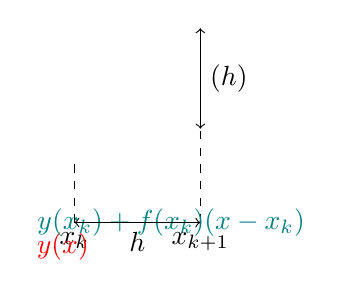
\begin{tikzpicture}[scale=2]
    \def\StartX {0.3};
    \draw [dashed] (\StartX,0) node[below]{$x_k$} -- (\StartX,{exp(\StartX*\StartX-1)});
    \draw [domain=0:2, range=0:2,color=red] plot function{exp(x*x-1)} node[anchor=north west]{$y{(x)}$};

    \def\EndX {1.1};
    \draw [dashed] (\EndX,0) node[below]{$x_{k+1}$} -- (\EndX,{+exp(\EndX*\EndX-1)});
    \draw [domain=0:\EndX, color=teal,thick] plot function{exp(\StartX*\StartX-1)+2*exp(-1 + \StartX*\StartX)*\StartX*(x-\StartX)} node[right]{$y(x_k)+f(x_k)(x-x_k)$};
    \draw [<->] (\EndX,{exp(\StartX*\StartX-1)+2*exp(-1 + \StartX*\StartX)*\StartX*(\EndX-\StartX)}) -- node[right]{$\bigO(h)$} (\EndX, {exp(\EndX*\EndX-1)});
    \draw [<->] (\StartX, 0) --node[below]{$h$} (\EndX, 0);
  \end{tikzpicture}
  \caption{Пример явного метода Эйлера}
\end{figure}

\subsubsection*{Неявный метод Эйлера}

Разностная схема получается из пункта 2) доказанной выше леммы:
\[\frac{y_{k+1}-y_k}{h}= f(x_{k+1},y_{k+1}) + \bigO(h),\ y_0=y(x_0)\]
Локальная погрешность $O(h^2)$, глобальная погрешность и сходимость $O(h)$.
Является более устойчивой схемой, чем явный метод Эйлера.

\begin{figure}[h]
  \centering
  \tikzsetnextfilename{13/ImplicitEuler}
  \begin{tikzpicture}[scale=2]
    \def\StartX {0.3};
    \draw [dashed] (\StartX,0) node[below]{$x_k$} -- (\StartX,{exp(\StartX*\StartX-1)});
    \draw [domain=0:2, range=0:2,color=red] plot function{exp(x*x-1)} node[anchor=north west]{$y{(x)}$};

    \def\EndX {1.1};
    \draw [dashed] (\EndX,0) node[below]{$x_{k+1}$} -- (\EndX,{+exp(\EndX*\EndX-1)});
    \draw [domain=0:4, range=0:2.8, color=teal, thick] plot function{exp(\StartX*\StartX-1)+2*exp(-1 + \EndX*\EndX)*\EndX*(x-\StartX)} node[right]{$y(x_k)+f(x_{k+1})(x-x_k)$};
    \draw [domain=0:2, range=0:2, color=darkgray, dashed] plot function{exp(\EndX*\EndX-1)+2*exp(-1 + \EndX*\EndX)*\EndX*(x-\EndX)} node[right]{$y(x_{k+1})+f(x_{k+1})(x-x_{k+1})$};
    \draw [<->] (\EndX,{exp(\StartX*\StartX-1)+2*exp(-1 + \EndX*\EndX)*\EndX*(\EndX-\StartX)}) -- node[anchor=south west]{$\bigO(h)$} (\EndX, {exp(\EndX*\EndX-1)});
    \draw [<->] (\StartX, 0) --node[below]{$h$} (\EndX, 0);
  \end{tikzpicture}
  \caption{Пример неявного метода Эйлера}
\end{figure}

Неявный метод называется именно так из-за того, что разностное уравнение
в схеме является нелинейным. Для того, чтобы его решать предлагается
вводить внутренний итерационный процесс
\[y_{k+1}^{j+1}= y_k+hf(x_{k+1},y_{k+1}^{j}),\ y_{k+1}^{0}=y_{k}\]
При достаточно малых $h$ и достаточно гладкой $f$ можно показать,
что данное отображение является сжимающим.

\subsection*{Методы Адамса второго порядка точности}

\subsubsection*{Через формулу прямоугольника по средней точке}
Из пункта 3) доказанной выше леммы получили следующую оценку
\[y(x_k+h)=y(x_k)+hf(y(x_k+h/2), x_k+h/2)+\bigO(h^3)\]
Но в пространстве $Y_h$ не определен узел $x_k+h/2$, поэтому
для расчетной формулы нужно думать что-то другое.

Один из вариантов: представить $y(x_k+h/2):=\frac{y(x_k)+y(x_k+h)}{2}$ и
воспользоваться снова итерационным процессом для расчетной
формулы $y_{k+1}=y_{k}+hf(\frac{y_k+y_{k+1}}{2}, x_k+h/2)+\bigO(h^3)$.

Рассмотрим другой вариант: пусть $\exists\ y_{k+1/2}^*\defeq y_k+\bigO(h^2)$, тогда
мы можем записать расчетную формулу следующим образом:
\begin{multline*}
  y_{k+1}=y_{k}+hf(y_k, x_k+h/2)\pm hf(x_k+h/2,y_{k+1/2}^*)+\bigO(h^3)= \\
  = y_{k}+hf(x_k+h/2,y_{k+1/2}^*)+ (hf(y_k, x_k+h/2)-hf(x_k+h/2,y_{k+1/2}^*))+\bigO(h^3)
\end{multline*}
Воспользуемся теоремой о среднем: $\tilde{y_k}$ - точка между $y_{k+1/2}^*$ и $y_k$
\[y_{k+1}= y_{k}+hf(x_k+h/2,y_{k+1/2}^*)+ \frac{h}{2}(f_x(\tilde{y_k}, x_k+h/2))\underbrace{(y_{k+1/2}^*-y_k)}_{\bigO(h^2)}+\bigO(h^3)=y_{k}+hf(x_k+h/2,y_{k+1/2}^*)+\bigO(h^3)\]
Точку $y_{k+1/2}^*$ можно посчитать с помощью явного метода Эйлера,
который как раз и обеспечивает второй порядок сходимости $y_{k+1/2}^*=y_k+\frac{h}{2}f(x_k,y_k)$
Итоговая расчетная форумла
\[\begin{cases}
    y_{k+1/2}^*=y_k+\frac{h}{2}f(x_k,y_k) \\
    y_{k+1}=y_{k}+hf(x_k+h/2,y_{k+1/2}^*) \\
    y_0=y(x_0)
  \end{cases}\]

\begin{figure}[h]
  \centering
  \tikzsetnextfilename{13/ImplicitAdamsMidPoint}
  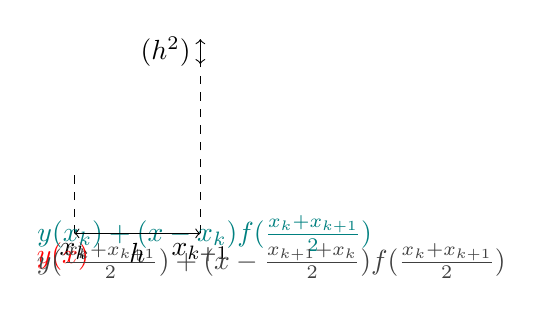
\begin{tikzpicture}[scale=2]
    \def\StartX {0.3};
    \draw [dashed] (\StartX,0) node[below]{$x_k$} -- (\StartX,{exp(\StartX*\StartX-1)});
    \draw [domain=0:2, range=0:2,color=red] plot function{exp(x*x-1)} node[anchor=north west]{$y{(x)}$};

    \def\EndX {1.1};
    \draw [dashed] (\EndX,0) node[below]{$x_{k+1}$} -- (\EndX,{+exp(\EndX*\EndX-1)});
    \draw [domain=0:1.3, color=teal,thick] plot function{exp(\StartX*\StartX-1)+2*exp(-1 + (\StartX+\EndX)**2/4)*(\StartX+\EndX)*(x-\StartX)/2} node[right]{$y(x_k)+(x-x_k)f(\frac{x_k+x_{k+1}}{2})$};
    \draw [domain=0:1.3, color=darkgray, dashed] plot function{exp(((\StartX+\EndX)**2)/4-1)+2*exp(-1 + (\StartX+\EndX)**2/4)*(\StartX+\EndX)*(x-(\EndX+\StartX)/2)/2} node[anchor=north west]{$y(\frac{x_k+x_{k+1}}{2})+(x-\frac{x_{k+1}+x_k}{2})f(\frac{x_k+x_{k+1}}{2})$};
    \draw [<->] (\EndX,{exp(\StartX*\StartX-1)+2*exp(-1 + (\StartX+\EndX)^2/4)*(\StartX+\EndX)*(\EndX-\StartX)/2}) -- node[left]{$\bigO(h^2)$} (\EndX, {exp(\EndX*\EndX-1)});
    \draw [<->] (\StartX, 0) --node[below]{$h$} (\EndX, 0);
  \end{tikzpicture}
  \caption{Пример неявного метода Адамса через среднюю точку}
\end{figure}

Через точку $x_k$ проводится касательная с углом наклона,
равным коэффициенту касательной, построенной по явному методу Эйлера через среднюю точку.

\subsubsection*{Через формулу трапеции}
Разностная схема получается из пункта 4) доказанной выше леммы:
\[y_{k+1}=y_k+h\frac{f(x_k,y_k)+f(x_{k+1},y_{k+1})}{2}+\bigO(h^3)\]
Схема получается нелинейная, для решения можно воспользоваться итерационным
методом. Мы воспользуемся аналогично формуле прямоугольника по центральной
точке хитростью.

Пусть $\exists\ y_{k+1}^*\defeq y_k+\bigO(h^2)$, тогда
мы можем записать расчетную формулу следующим образом:
\begin{multline*}
  y_{k+1}=y_k+h\frac{f(x_k,y_k)+f(x_{k+1},y_{k+1})}{2}\pm\frac{h}{2}f(x_{k+1},y_{k+1}^*)+\bigO(h^3)= \\
  = y_k+h\frac{f(x_k,y_k)+f(x_{k+1},y_{k+1}^*)}{2}+\frac{h}{2}(f(x_{k+1},y_{k+1})-f(x_{k+1},y_{k+1}^*))+\bigO(h^3)
\end{multline*}
Воспользуемся теоремой о среднем: $\tilde{y_k}$ - точка между $y_{k+1}^*$ и $y_k$
\begin{multline*}
  y_{k+1}=y_k+h\frac{f(x_k,y_k)+f(x_{k+1},y_{k+1}^*)}{2}+\frac{h}{2}f_x(x_{k+1},\tilde{y_k})\underbrace{(y_{k+1}^*-y_k)}_{\bigO(h^2)}+\bigO(h^3)= \\
  =y_k+h\frac{f(x_k,y_k)+f(x_{k+1},y_{k+1}^*)}{2}+\bigO(h^3)
\end{multline*}
Точку $y_{k+1}^*$ будем искать с помощью явного метода Эйлера $y_{k+1}^*=y_k+hf(x_k,y_k)$.
Итоговая расчетная формула
\[\begin{cases}
    y_{k+1}^*=y_k+hf(x_k,y_k)                                         \\
    y_{k+1}=y_k+h\frac{f(x_k,y_k)+f(x_{k+1},y_{k+1}^*)}{2}+\bigO(h^3) \\
    y_0=y(x_0)
  \end{cases}\]

\begin{figure}[h]
  \centering
  \tikzsetnextfilename{13/ImplicitAdamsTrapezoid}
  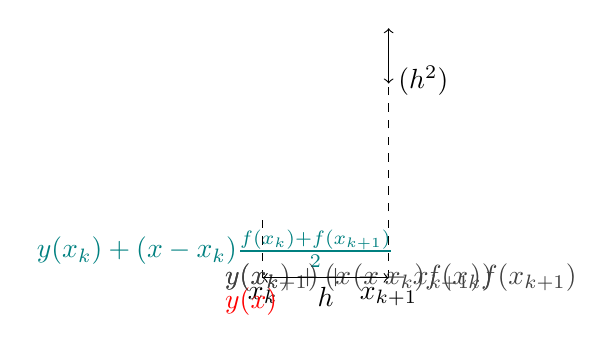
\begin{tikzpicture}[scale=2]
    \def\StartX {0.3};
    \draw [dashed] (\StartX,0) node[below]{$x_k$} -- (\StartX,{exp(\StartX*\StartX-1)});
    \draw [domain=0:2, range=0:2,color=red] plot function{exp(x*x-1)} node[anchor=north west]{$y{(x)}$};

    \def\EndX {1.1};
    \draw [dashed] (\EndX,0) node[below]{$x_{k+1}$} -- (\EndX,{+exp(\EndX*\EndX-1)});
    \draw [domain=0:1.3, color=teal,thick] plot function{exp(\StartX*\StartX-1)+(exp(-1 + \StartX*\StartX)*\StartX+exp(-1 + \EndX*\EndX)*\EndX)*(x-\StartX)} node[above]{$y(x_k)+(x-x_k)\frac{f(x_k)+f(x_{k+1})}{2}$};
    \draw [domain=0:1.3, range=0:2, color=darkgray, dashed] plot function{exp(\StartX*\StartX-1)+(2*exp(-1 + \StartX*\StartX)*\StartX)*(x-\StartX)} node[right]{$y(x_k)+(x-x_k)f(x_k)$};
    \draw [domain=0:1.3, range=0:2, color=darkgray, dashed] plot function{exp(\EndX*\EndX-1)+(2*exp(-1 + \EndX*\EndX)*\EndX)*(x-\EndX)} node[right]{$y(x_{k+1})+(x-x_{k+1})f(x_{k+1})$};
    \draw [<->] (\EndX,{exp(\StartX*\StartX-1)+(exp(-1 + \StartX*\StartX)*\StartX+exp(-1 + \EndX*\EndX)*\EndX)*(\EndX-\StartX)}) -- node[anchor=north west]{$\bigO(h^2)$} (\EndX, {exp(\EndX*\EndX-1)});
    \draw [<->] (\StartX, 0) --node[below]{$h$} (\EndX, 0);
  \end{tikzpicture}
  \caption{Пример неявного метода Адамса через формулу трапеции}
\end{figure}

Через точку $x_k$ проводится касательная с углом наклона,
равным среднему арифметическому коэффициентов
касательных, построенных по явному и неявному методам Эйлера.

\begin{remark}
  Предложенные варианты с заменой на явные методы Эйлера облегчают
  подсчет итоговой расчетной формулы, но при этом отрицательно влияют на устойчивость
  задачи.
\end{remark}
